\documentclass[11pt,a4paper]{article}
\usepackage[hyperref]{acl2018}
\usepackage{times}
\usepackage{latexsym}

%\aclfinalcopy % Uncomment this line for the final submission
%\def\aclpaperid{***} %  Enter the acl Paper ID here

%\setlength\titlebox{5cm}
% You can expand the titlebox if you need extra space
% to show all the authors. Please do not make the titlebox
% smaller than 5cm (the original size); we will check this
% in the camera-ready version and ask you to change it back.


\usepackage{graphicx} % for imports
\usepackage{subcaption} % for figures
\usepackage{cleveref}
\graphicspath{{img/}}
%\usepackage{wrapfig} % Used for prettier figures
\usepackage{pgfplots} % plotting pgf format directly
% citations

\title{Planning Paper}

\author{Luis Glaser\\
  Matrikelnumber 800140 \\
  Potsdam University \\
  {\tt Luis.Glaser@uni-potsdam.de}
  \\}

\date{}
\usepackage{url}

\begin{document}
\maketitle
\begin{itemize}
\item What is your project about and what approach are you going to take?
\item What tools and/or data will you use?
\item What will you learn from this project? How does the successful imple- mentation of the project help you achieve the learning objectives of the class?
\item What will be your personal role in the team, which skills and what knowl- edge can you contribute?
\end{itemize}


\section{Introduction \& Motivation}

Together with Atreya Shankar and Juliane Hanel I will work on music lyrics. The original motivation was our shared interest in music and the different cultural dimension it expresses. And we were interested whether we would be able to find patterns only in the lyrical data when excluding the acoustic part. Some of these initial questions where if there's a difference between rap and pop lyrics, how they differ in emotionality and how music lyrics in general have evolved over time.
This planning paper serves the purpose of structuring those initial questions, in order to keep our research focused. This will happen in k% TODO: FIX
 steps. First what data we will use, because this already will restrict the possible questions we can pose. 

\section{State of the Art}

\section{Method}
\begin{figure}[h]
	\centering
	\resizebox{\linewidth}{!}{
		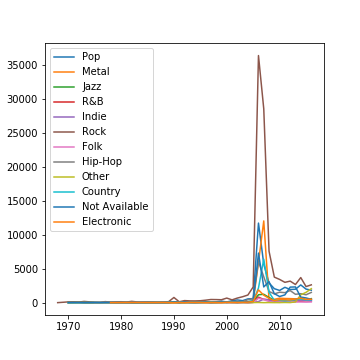
\includegraphics{img/kaggleplot_bias}
	}
	\caption{Distribution of genre over time in \texttt{kaggle} data}
       \label{fig:kaggle}
\end{figure}
% Data
When first experimenting with our approach, we went with the first available data set from %TODO cite kaggle shit
However, we came across initial flaws, as the dataset was very biased towards a certain year. This can easily be seen in the histogram depicted in \cref{fig:kaggle} we will not use this in the end. We currently have two approaches we could take from here. The first one will be to crawl data by ourselves by interfacing with the genius API.\footnote{\url{https://docs.genius.com}}
This is still in progress and we can't yet decide if this dataset will have less of a bias. The second technique will be to search for further datasets and integrate them into one dataset. This would have multiple disadvantages. First, it's likely that we won't be able to completely get rid of the bias and second will introduce new challenges like merging the data and unifying their formats. This wouldn't provide anything interesting for us to learn. 

\section{Tooling}
\begin{figure}[h!]
	\centering
	\scriptsize
	\begin{tabular}{llllll}
ID & Artist & Title & Year & Genre & Lyrics \\
1 & Rihanna & Diamonds & 2012 & Pop & Shine bright $\ldots$ \\
	\end{tabular}
	\caption{Example entries in \texttt{SQLite} database}
	\label{fig:table}
\end{figure}
For data house keeping we'll use a \texttt{SQLite}\footnote{\url{https://www.sqlite.org}} database which will be shared over \texttt{GitHub} and interfaced via \texttt{python}. Furthermore as mentioned already in our group contract, we will use this \texttt{GitHub} repository for collaboration in general. 

In both cases we will scrutinize % WORT richtig?
our data for any irregularities or unforseen biases and .. mach ma hoit wos mit ean.


\section{Personal Contribution}

I will contribute to this project on multiple different ends. 

I will be responsible of taking care of our database system. In both my undergraduate degrees I had had to work with rather large datasets that kept changing during work. Thus, I am familiar with a few pitfalls concerning data handling. My work should ensure that all of us can work undisrupted and not have to bother a lot with the usual data juggling. 

\section{Learning Goals}

Our project will use quite a few techniques that were not discussed in class. However we hope that using those techniques will give us not the ability to apply the knowledge and methods we learned in class on another project. We also will be able to try out new methds which will help me / us when deciding of the further classes to take during the masters programm. Or if I should drop this shit entirely and go for computer science lel



\bibliographystyle{acl}
\bibliography{bibtex}



\end{document}

